
\chapter{Introduction}


Agriculture and its allied sectors in India accounted for 17-18\% of the GDP(Gross Domestic Product) in 2018 \cite{stats1}. India ranks first globally with the highest net crop area\cite{stats2}. It has a majority of its total land's occupancy, reported being 60.45\% with a total land area of 159.7 million hectares (394.6 million acres), invested in agriculture and related practices. It also had a massive human resource involvement of over 50\% reported in 2018 itself \cite{stats1}.
\\ 

With this big of traction in the economic contribution and resource utilization, the agricultural sector is still suffering due to very little or no involvement of technology whatsoever, among other natural factors. Farmers rely on rudimentary methods and intention based inspection to analyse and act upon their crop fields' health. There is a very little contribution by the government to make a technical inclusion in the agricultural sector. This is attributed to its heavy investment in solving middlemen crisis, inflation rise and a sudden reduction in manpower in the sector due to the emergence and increase in awareness of newer sectors and digital transformations in the country which is impending a paradigm shift.
\\

In our study, we focus on the areas of field analysis in the agroforestry domains to get insights on the crop field in a systematically efficient manner with sufficient resolution and act upon them at a larger level. The current field health analysis is done by farmers manually using rudimentary techniques wherein they do a manual inspection of their complete fields. This, without any special aids, is very time consuming and gives inaccurate results due to the raw analysis of chlorophyll levels and the inefficiency of farmer's knowledge in new crops. A very bleak section of farmers benefit from technical aids. However, most of these systems use satellite imagery for assessing the plant health. The satellite based systems rely on a small public data gathered by a limited number of satellites. These have a very low rate of revisiting of the field due to their Low Earth Orbits and small number of satellites employed for the purpose. They also are able to provide only coarse spatial resolutions of about 5 meters per pixel which are inefficient at miniature levels. Further, they can only work with the Area of Interest (AOI) if the cloud coverage is less than 5\% \cite{eighth}. The satellite based method is also inaccessible in a user-friendly format. Hence, the satellite based method causes major feasibility issues in India where these problems are persistent and relying completely on satellite systems leaves us confined to several constraints of availability in spite of providing a band rich multi-spectra as well as hyperspectral imaging in the captured data.
\\

Therefore we propose a UAS (Unmanned Aerial Vehicle) based solution which could work more accurately with high degrees of spatial resolution, does not rely on public data for non-learning based results, is not confined by cloud coverages and can be presented to the farmers as a service for the complete analysis of their agricultural fields, eliminating the need of time-consuming and inaccurate manual inspection of fields for the yield prediction, smarter farming practices and health assessments. The solution is called as Dronalyser, which is a drone-based service for the agricultural inspection of the agricultural crop fields. The service has the following parts:




\begin{figure}[H]
    \centering
    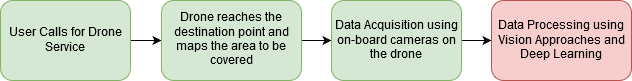
\includegraphics[width=\linewidth]{SummerInterReport/project/Images-Major/Intro_Flow.png}
    \caption{A concise flow of the proposed idea}
    \label{fig:Concise Flow}
\end{figure}

\section{Overview}

Our work compiles a study and explores various developments of a multispectral processing system based on an UAS (Unmanned Aerial System) to perform analysis on agricultural fronts and enable farmers to use smart precision farming. A quadcopter (drone) is used as the UAS where it covers the area based on a service call from the application. The imagery part is achieved by an embedded system, Raspberry Pi, which does the data acquisition and data processing. A modified one camera setup of the NoIR (No InfraRed Filter CMOS sensor) camera has been used for capturing the aerial imagery for computation. A comparative camera study was also performed. The data processing involved comparison of reflectances of Near IR and Red spectra to calculate the NDVI and thereby assess the plant health.


\section{Calling for Drone Service}
An android application serves as the user end application part of the system. It can be used in either Hindi or English to call for the drone service. The application has an easy to use interface where the farmer's phone gets registered automatically as a user and the farmer can call for the drone at his own position using the phone's GPS location. The application allows the user to fetch previous reports from the Firebase storage database or analyze live status of the field analysis over LAN (Local Area Network) connection to the drone in close proximity. In case the farmer doesn't have a smartphone, the system uses Twilio server on python backend for the drone dispatch stations using which, a farmer can send a SMS in a specified format, in which case the service would offer a personnel for operating the drone and presenting the reports to the farmer.
\section{Drone Mapping the area} The drone covers the area autonomously by stably following the geo-location tags based based on GPS computed for its path by the mission planner. We used the ArduPilot APM 2.8 flight controller which has an embedded firmware for stabilizing the drone using various flight modes after callibrating it, analyzing its flight metrics, GPS integration and support for external compass, I2C and telemetry as well. The APM was programmed using open-source software, the firmware ArduCopter 5.3.3 uploaded through Mission Planner based on ArduPilot platform, to first follow the GPS tag to the Field location from the nearest Base Station and then covering the complete area through covering the polygon drawn over the field to be covered or Area Of Interest (AOI) by the path computed.

\section{Data Acquisition} The data acquisition system consists of a Raspberry Pi, A NoIR Pi camera and the trigger from the APM. An open source plugin in Mission Planner, OperDroneMap(ODM) was used to merge the multi-spectral imagery into an orthomosaic from the captured images. 

\section{Data Processing} The data is processed as live time feed of the drone imagery where every frame is computed to yield the infographic feed and the post processing involves combining the individual frames into an orthomosaic covering the entire field using an open source software Fiji or using mathematical modelling of the distance. A developed Python script calculates the Normalized Difference Vegetation Index (NDVI) through the Near InfraRed (NIR) and Red field reflectance spectra collected from the NoIR Pi camera, acting as a metric to define the plant health through chlorophyll level analysis. This NDVI calculation is done both on the frame wise feed and the final orthomosaic. The complete information graphic developed lets the farmer know which areas of the field are poor in chlorophyll and thereby health. Also, we present a water index of the field using only the Near IR spectrum, which is a clear indicator of water's thermal coefficient and thereby the water retention in every region of the crop field. 


%stats1 citation - "India economic survey 2018: Farmers gain as agriculture mechanisation speeds up, but more R&D needed". The Financial Express. 29 January 2018.  https://www.financialexpress.com/budget/india-economic-survey-2018-for-farmers-agriculture-gdp-msp/1034266/

%stats2 citation- "India outranks US, China with world's highest net cropland area". Retrieved 17 November 2018. http://www.indiawaterreview.in/Story/Features/india-outranks-us-china-with-worlds-highest-net-cropland-area/2096/2#.W_A_iOgzZPY

%eighth- Multi Temporal Data wala